%!TEX root = booklet.tex

% start on even (left) page
% such that the 3x two schedule pages/days are adjacent to / facing eachother
% \ifthispageodd{}{}

~\cleardoublepage

\section{Schedule at a Glance}

% \vspace{-2mm}%

\ifodd\value{page}
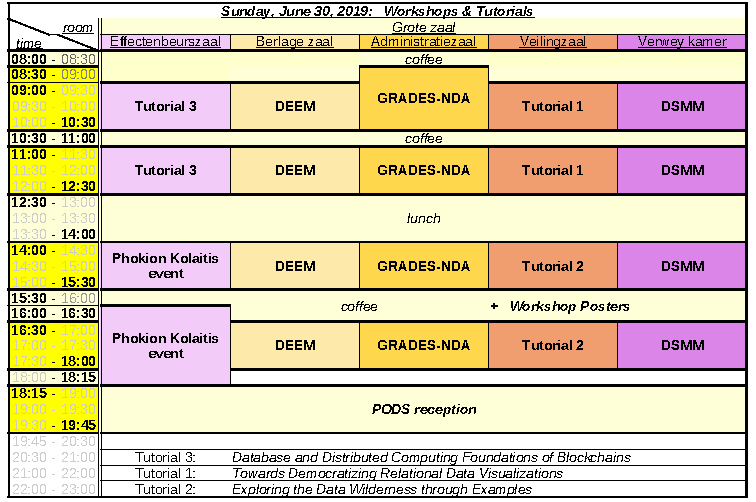
\includegraphics[height=\textwidth,width=.97\textheight,angle=90]{schedule/p1.pdf}%
\else
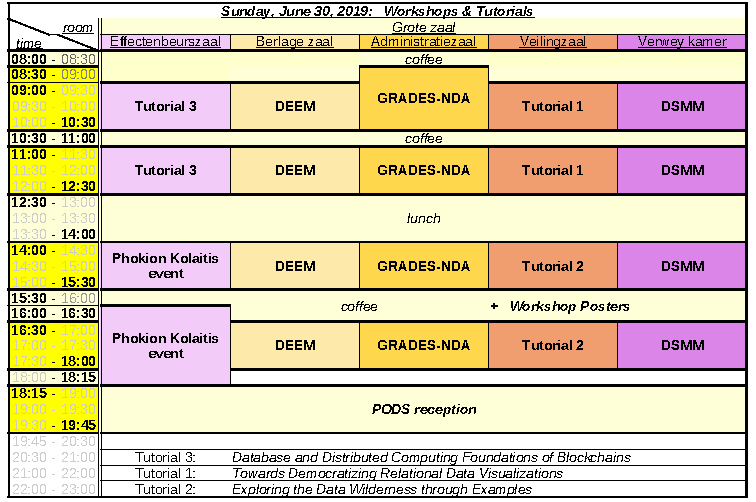
\includegraphics[height=\textwidth,width=.97\textheight,angle=270]{schedule/p1.pdf}%
\fi

\newpage

\vspace{-10mm}%

\ifodd\value{page}
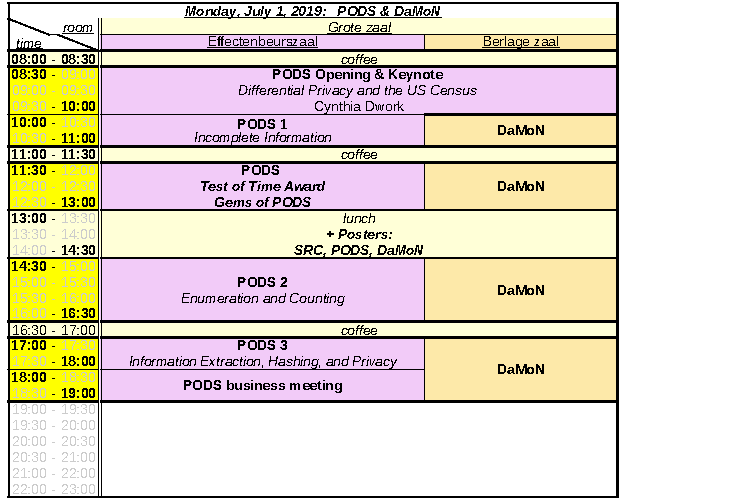
\includegraphics[angle=90,width=\textwidth]{schedule/p2.pdf}%
\else
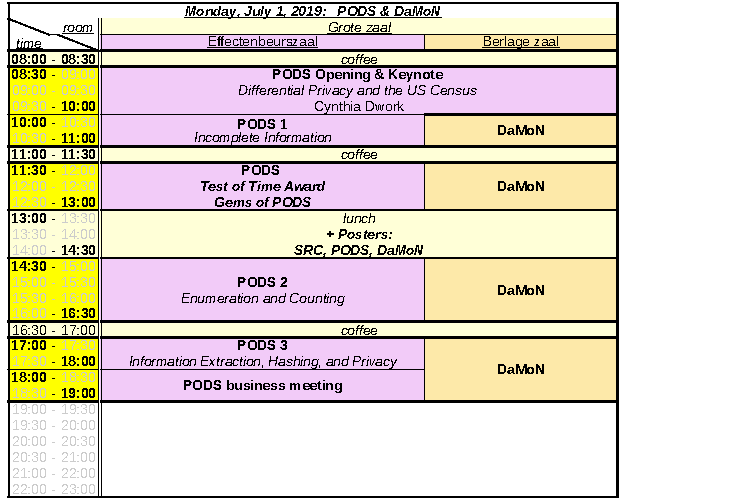
\includegraphics[angle=270,width=\textwidth]{schedule/p2.pdf}%
\fi

\newpage

\ifodd\value{page}
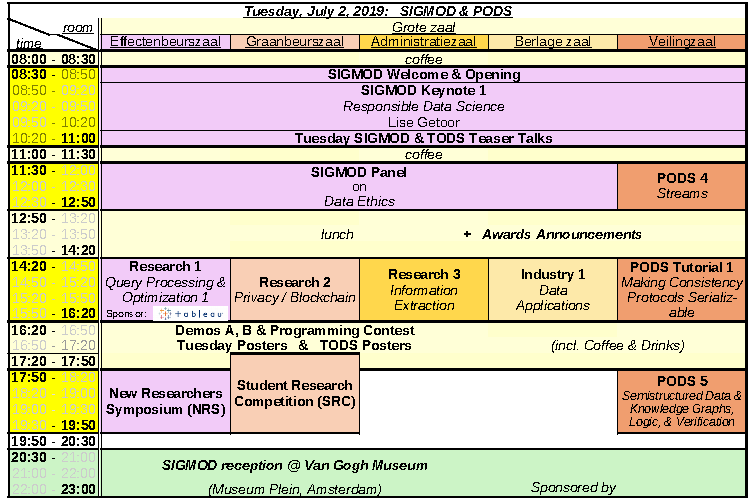
\includegraphics[angle=270,width=\textwidth]{schedule/p3.pdf}%
\else
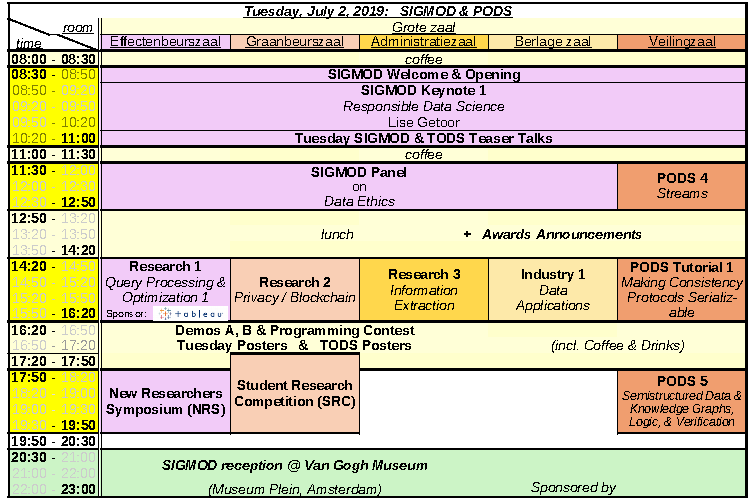
\includegraphics[angle=90,width=\textwidth]{schedule/p3.pdf}%
\fi

\newpage

\ifodd\value{page}
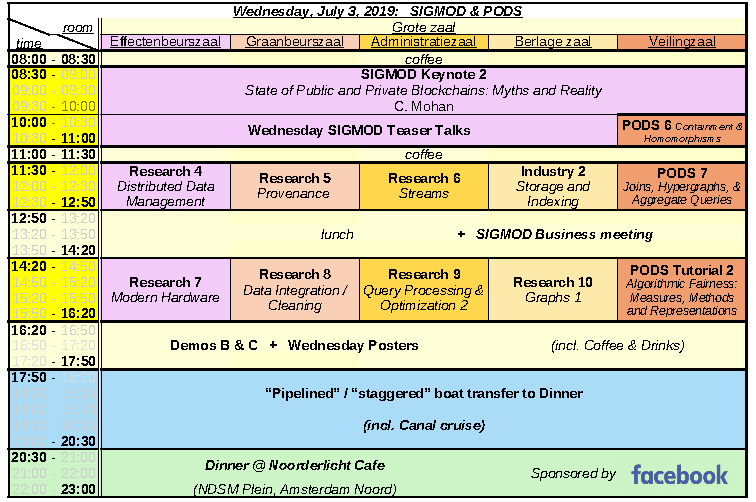
\includegraphics[angle=90,width=\textwidth]{schedule/p4.pdf}%
\else
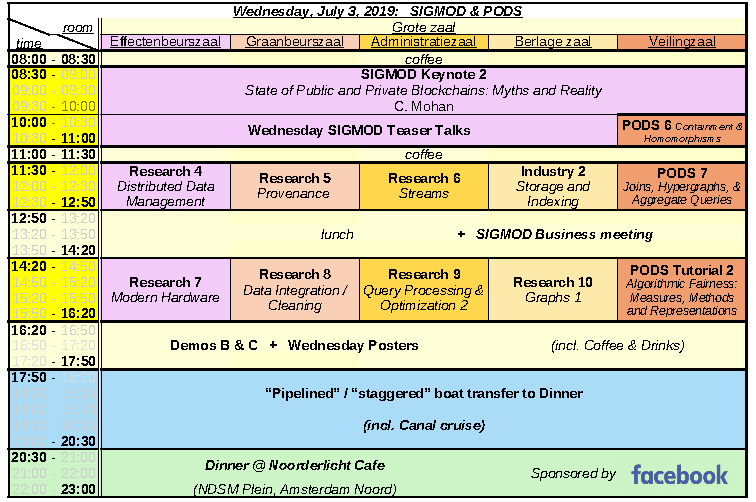
\includegraphics[angle=270,width=\textwidth]{schedule/p4.pdf}%
\fi

\newpage

\ifodd\value{page}
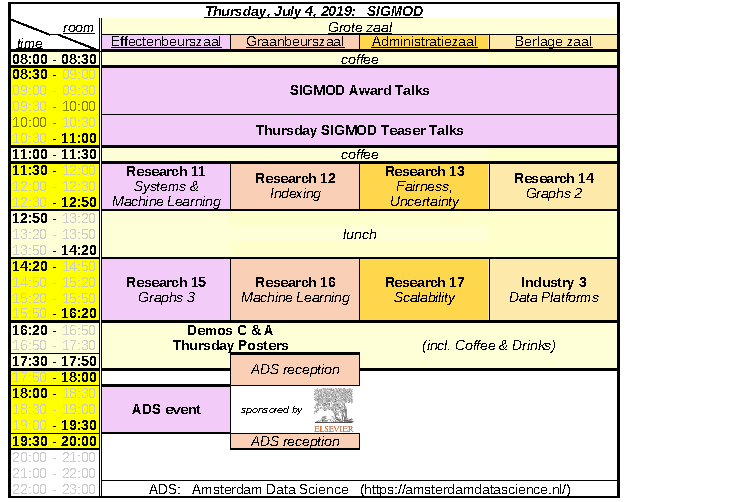
\includegraphics[angle=270,width=\textwidth]{schedule/p5.pdf}%
\else
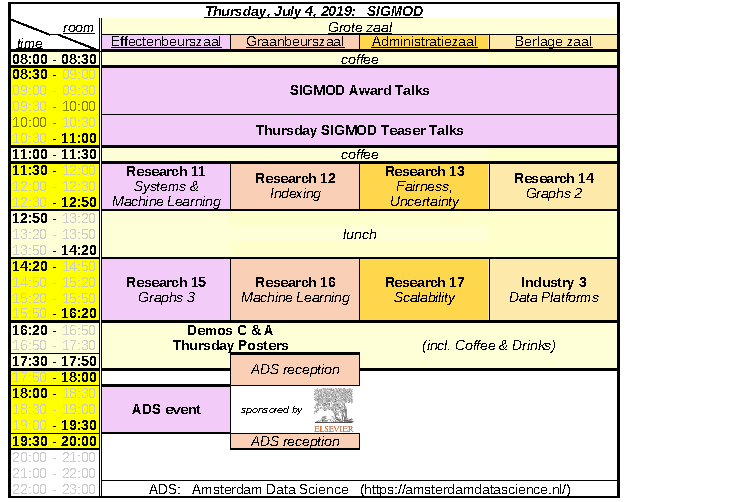
\includegraphics[angle=90,width=\textwidth]{schedule/p5.pdf}%
\fi

\newpage

\ifodd\value{page}
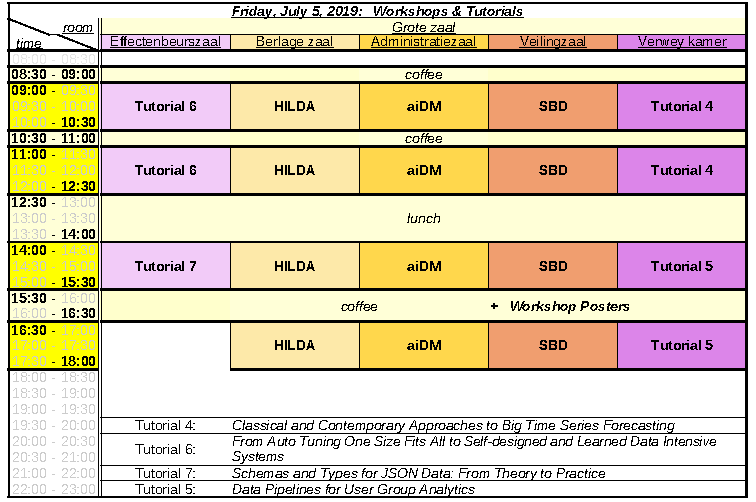
\includegraphics[angle=90,width=\textwidth]{schedule/p6.pdf}%
\else
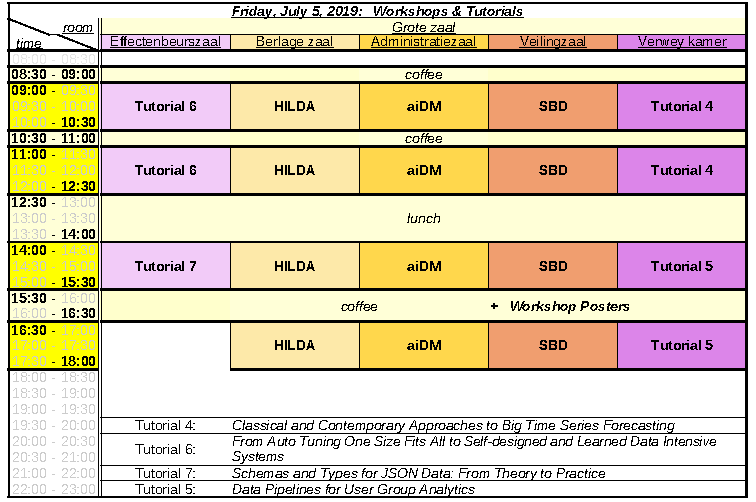
\includegraphics[angle=270,width=\textwidth]{schedule/p6.pdf}%
\fi






